\documentclass{beamer}
\usepackage[utf8]{inputenc}
\usepackage[spanish]{babel}
\usetheme{metropolis} 

%Listas
\usepackage{listings}
\usepackage{enumerate}
\usepackage{enumitem}

% Varias columnas
\usepackage{multicol}

\usepackage[default]{sourcesanspro}

\usepackage{hyperref}
\hypersetup{
    colorlinks=true,
    linkcolor=black,
    urlcolor=blue,
    citecolor=blue,
}

% Paquete para citas literales
\usepackage{dirtytalk}

%Cambiar el tamaño de los comentarios de las figuras
\usepackage[font=footnotesize,labelformat=empty]{caption}

% Desactivar un warning del paquete Hyperref
\pdfstringdefDisableCommands{
  \def\\{}
}

\title{Reimplementación de videojuegos clásicos en Three.js utilizando técnicas de generación procedimental}
\author{
    \textbf{Autor:} Guillermo Sandoval Schmidt\\
    \textbf{Director:} Francisco Velasco Anguita
}
\institute[UGR]{Universidad de Granada\\
\medskip
\url{https://github.com/Gsandoval96/TFG-UGR}
}
\date{23 de noviembre de 2021}

\begin{document}

\setbeamercolor{background canvas}{bg=white} %cambiamos el color de fondo a blanco

\maketitle

\setbeamertemplate{section in toc}[ball unnumbered]
\begin{frame}{Índice}
    \tableofcontents
\end{frame}

\AtBeginSection[ ]
{
\begin{frame}{Índice}
    \tableofcontents[currentsection]
\end{frame}
}

\section{Introducción}

    \begin{frame}{Motivación \scriptsize{\hfill \secname}}
        \begin{itemize}
        \item El interés por aprender sobre generación procedimental de contenido aplicada a videojuegos.
        \item La afición y admiración por los videojuegos clásicos originarios de las máquinas arcade de los años 80.
        \item La intención de mejorar el aprendizaje sobre desarrollo de videojuegos a más bajo nivel.
    \end{itemize}
    \end{frame}

    \begin{frame}{Objetivos \scriptsize{\hfill \secname}}
    
    \begin{itemize}
        \item La investigación y el autoaprendizaje sobre generación procedimental de contenidos.
        \rule{9cm}{0.4pt}
        \item La aplicación de generación procedimental de contenidos a videojuegos clásicos, aplicando diversas técnicas.
        \item La reimplementación del videojuego clásico Pac-Man utilizando técnicas de bajo nivel y sin la ayuda de un motor de videojuegos.
    \end{itemize}
        
    \end{frame}

\section{Planificación}

    \begin{frame}{Diagrama de Gantt - abril a julio \scriptsize{\hfill \secname}}
        \begin{figure}[H]
        \centering
            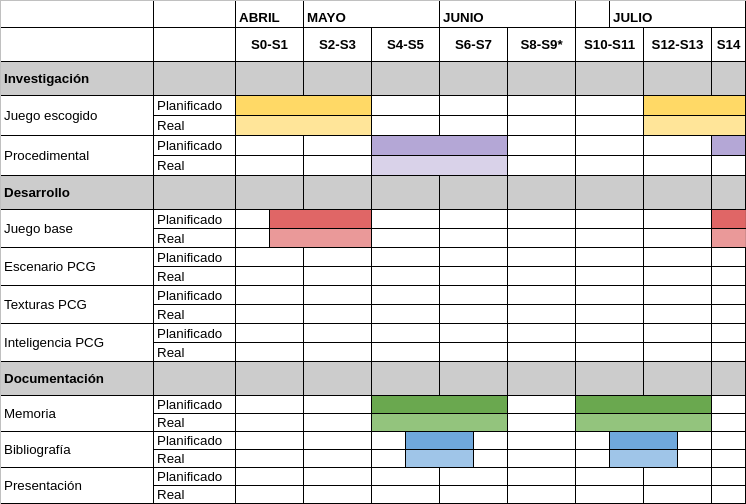
\includegraphics[scale=0.375]{img/gantt-A.PNG}
        \end{figure}
    \end{frame}
    
    \begin{frame}{Diagrama de Gantt - agosto a noviembre \scriptsize{\hfill \secname}}
        \begin{figure}[H]
        \centering
            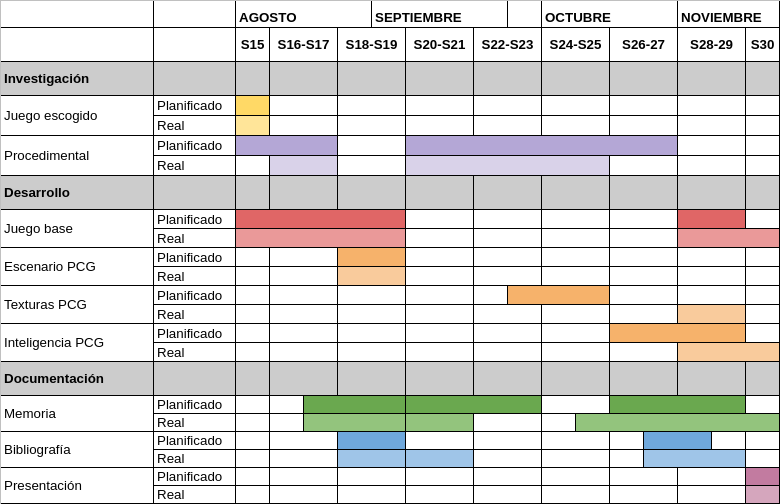
\includegraphics[scale=0.375]{img/gantt-B.PNG}
        \end{figure}
    \end{frame}

\section{Estado del arte}

    \begin{frame}{Definición \scriptsize{\hfill \secname}}
    
    \say{\textit{El uso de un algoritmo formal para generar contenido [...] que normalmente sería producido por un humano}} \cite{smith2015}.
        
    \end{frame}
    
    \begin{frame}{Clasificación de contenido \scriptsize{\hfill \secname}}
    
    \begin{itemize}
        \item \textbf{Game Bits:} texturas, sonidos, vegetación...
        \item \textbf{Game Space:} mapeado o terreno.
        \item \textbf{Game Systems:} ecosistemas, comportamiento de entidades...
        \item \textbf{Game Scenario:} puzzles, niveles, historia...
        \rule{9cm}{0.4pt}
        \item \textbf{Game Desing:} mecánicas y reglas de juego.
        \item \textbf{Derived Content:} publicidad, post de páginas web, rankings...
    \end{itemize}
    
    \bigskip
    
    \scriptsize{Clasificación siguiendo los trabajos de \cite{hendrikx2013} y \cite{barriga2019}.}
        
    \end{frame}
    
     \begin{frame}{PCG en los videojuegos \scriptsize{\hfill \secname}}
    
    	\begin{table}[H]
    	\centering
    	\resizebox{\textwidth}{!}{%
    	\begin{tabular}{cc}
    	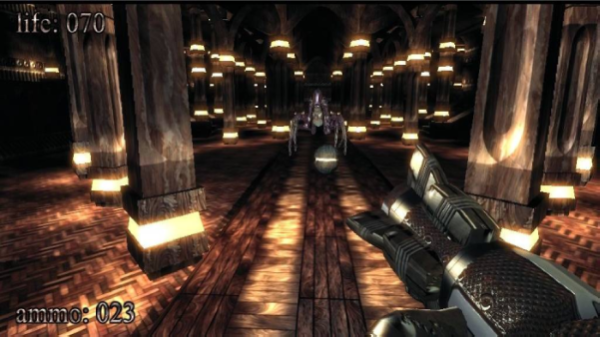
\includegraphics[width=0.25\textwidth]{img/kkrieger.png} & 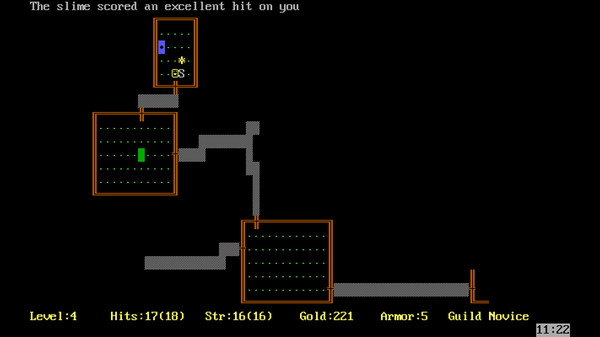
\includegraphics[width=0.25\textwidth]{img/rogue.png} \\
    	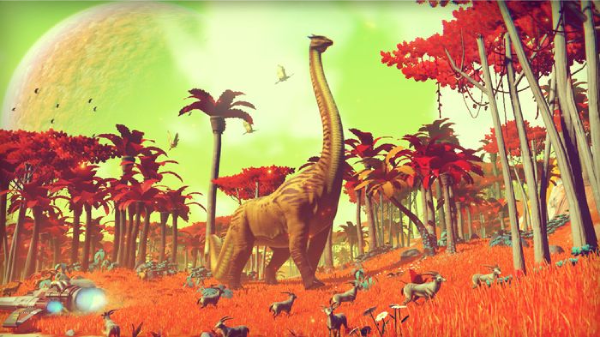
\includegraphics[width=0.25\textwidth]{img/no-mans-sky.png} & 
    	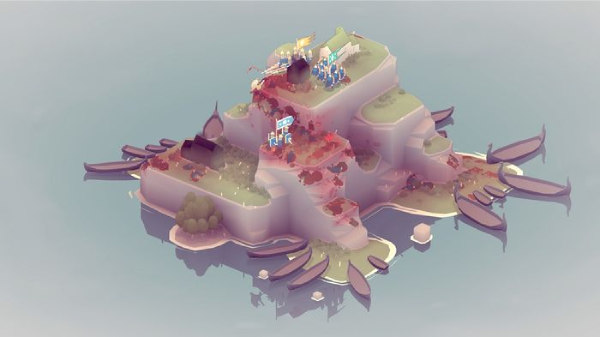
\includegraphics[width=0.25\textwidth]{img/bad_north.png} 
    	\end{tabular}%
    	}
    	\end{table}
    
    \end{frame}
    
    \begin{frame}{Propiedades deseables \scriptsize{\hfill \secname}}
    
        \begin{itemize}
            \item \textbf{Velocidad:} tiempo que tarda el algoritmo en generar contenido.
            \item \textbf{Fiabilidad:} precisión con la que garantiza el algoritmo que el contenido generado es de calidad.
            \item \textbf{Controlabilidad:} posibilidad de modificar o condicionar los resultados obtenidos.
            \item \textbf{Diversidad:} capacidad de generar contenido variado.
            \item \textbf{Credibilidad:} capacidad de imitar al contenido generado por humanos.
        \end{itemize}
        
        \bigskip
        
        \scriptsize{Clasificación siguiendo el libro de \cite{shaker2016}.}
        
    \end{frame}
    
    \begin{frame}{Clasificación de métodos \scriptsize{\hfill \secname}}
        \footnotesize{
        \begin{table}[H]
            \centering
            \begin{tabular}{|l|l|}
                \hline
                \textbf{Categoría}                         & \textbf{Métodos de PCG}                                                                                                                                          \\ \hline
                Métodos tradicionales             & \begin{tabular}[c]{@{}l@{}}Generación de números semi-aleatoria\\ Generación basada en fractales y ruido\\ Generación basada en gramáticas\end{tabular} \\ \hline
                Métodos basados en búsqueda       & Algoritmos evolutivos                                                                                                                                   \\ \hline
                Métodos de aprendizaje automático & \begin{tabular}[c]{@{}l@{}}Redes neuronales recursivas\\ Autoencoders\\ Modelos de Markov\end{tabular}                  \\ \hline
            \end{tabular}
        \end{table}
        }
        
        \bigskip
        
        \scriptsize{Clasificación siguiendo el trabajo de \cite{barriga2019}.}
        
    \end{frame}
    
    

\section{Análisis del problema}

\begin{frame}{Videojuego escogido: Pac-Man \scriptsize{\hfill \secname}}
    \begin{multicols}{2}
    
        \begin{itemize}
            \item \textbf{Objetivo:} Recorrer el laberinto comiéndonos todos los puntos mientras escapamos de los cuatro enemigos.
            \item \textbf{Jugador:} Pac-Man.
            \item \textbf{Enemigos:} Fantasmas.
            \item \textbf{Ayudas:} Potenciador o \textit{Power Pellet}.
            \item \textbf{Niveles:} Constan de un laberinto siempre con la misma distribución.
        \end{itemize}
        
        \begin{center}
            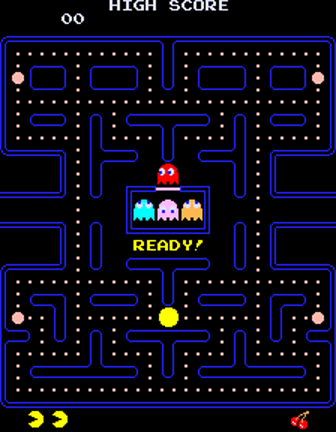
\includegraphics[scale=0.375]{img/lvl1.png}
            \scriptsize{Diseño de niveles del videojuego \textit{Pac-Man}. Imagen obtenida de \cite{pittman2015}.}
        \end{center}
        
        
        \end{multicols}
\end{frame}


\section{Implementación}

    \begin{frame}{Generación de laberintos \scriptsize{\hfill \secname}}
        \begin{figure}[H]
        \centering
            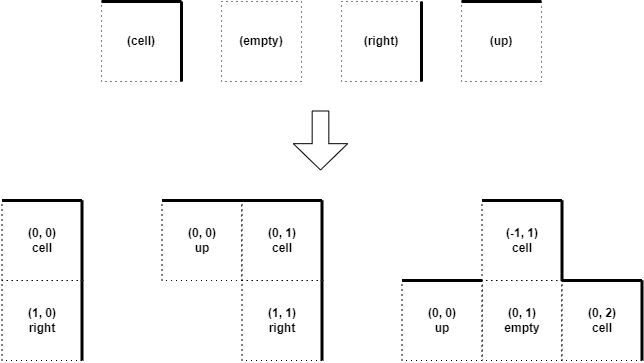
\includegraphics[scale=0.4]{img/celdasYpiezas.png}
        \end{figure}
    \end{frame}
    
    \begin{frame}{Generación de laberintos \scriptsize{\hfill \secname}}
        \begin{figure}[H]
        \centering
            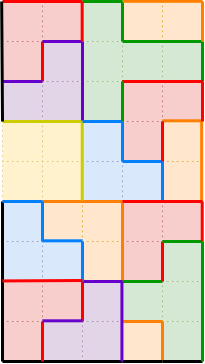
\includegraphics[scale=0.475]{img/grafo_color.png}
        \end{figure}
    \end{frame}

    \begin{frame}{Generación de laberintos - Modelo simple \scriptsize{\hfill \secname}}
        \begin{figure}[H]
        \centering
            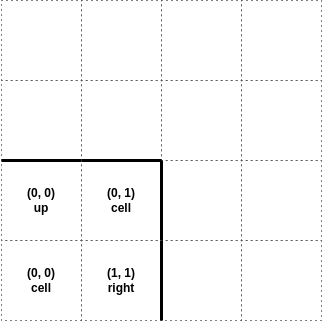
\includegraphics[scale=0.375]{img/paso1.png}
            \caption{\textbf{1.} Establecemos los valores de las casillas de la casa de los fantasmas.}
        \end{figure}
    \end{frame}
    
    \begin{frame}{Generación de laberintos - Modelo simple \scriptsize{\hfill \secname}}
        \begin{figure}[H]
        \centering
            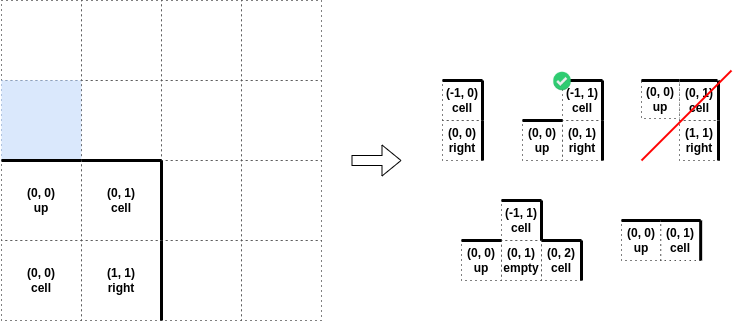
\includegraphics[scale=0.375]{img/paso2.png}
            \caption{\textbf{2.} Escogemos una casilla de la primera columna, seleccionamos una pieza de entre el conjunto de piezas válidas y la colocamos en nuestra matriz.}
        \end{figure}
    \end{frame}
    
    \begin{frame}{Generación de laberintos - Modelo simple \scriptsize{\hfill \secname}}
        \begin{figure}[H]
        \centering
            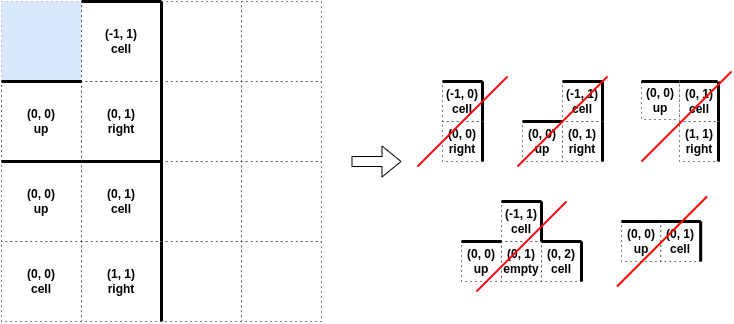
\includegraphics[scale=0.375]{img/paso3.png}
            \caption{\textbf{3.} Escogemos la única casilla restante de la primera columna. Al ir a seleccionar una pieza y estar vacío el conjunto de piezas válidas, rellenamos la casilla por defecto con una celda completa.}
        \end{figure}
    \end{frame}
    
    \begin{frame}{Generación de laberintos - Modelo simple \scriptsize{\hfill \secname}}
        \begin{figure}[H]
        \centering
            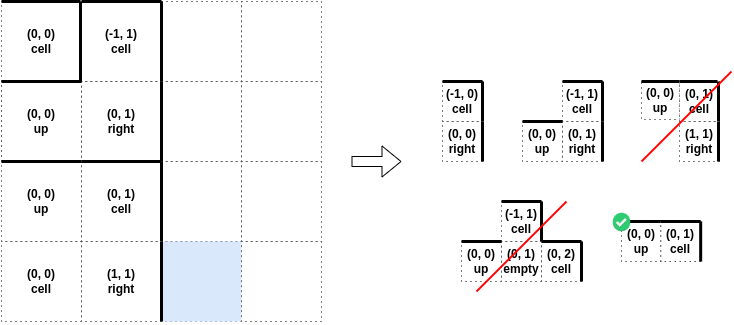
\includegraphics[scale=0.375]{img/paso4.png}
            \caption{\textbf{4.} Cambiamos a la tercera columna ya que la segunda ya está completa. Escogemos una casilla de la columna, seleccionamos una pieza entre las piezas válidas y la colocamos en nuestra matriz.}
        \end{figure}
    \end{frame}
    
    \begin{frame}{Generación de laberintos - Modelo simple \scriptsize{\hfill \secname}}
        \begin{figure}[H]
        \centering
            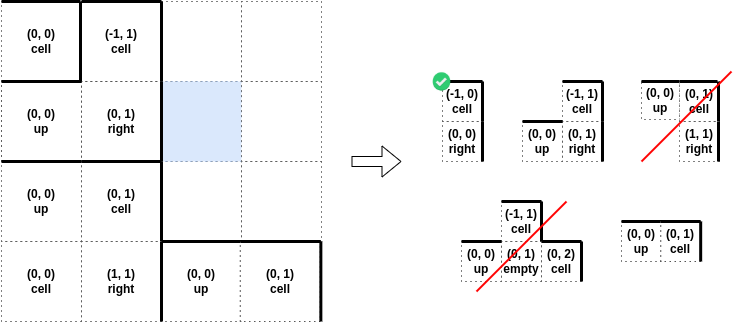
\includegraphics[scale=0.375]{img/paso5.png}
            \caption{\textbf{5.} Volvemos a repetir el paso anterior. Escogemos una casilla de la columna, seleccionamos una pieza entre las piezas válidas y la colocamos en nuestra matriz.}
        \end{figure}
    \end{frame}
    
    \begin{frame}{Generación de laberintos - Modelo simple \scriptsize{\hfill \secname}}
        \begin{figure}[H]
        \centering
            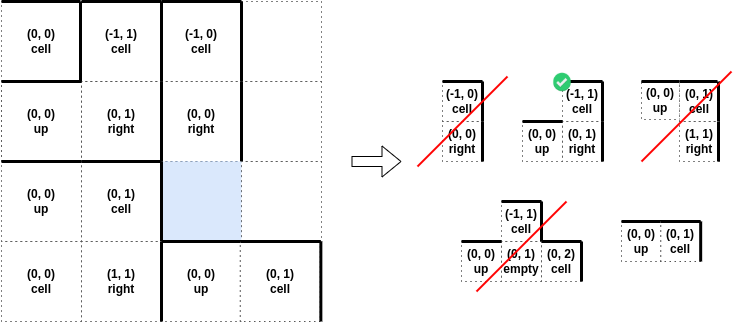
\includegraphics[scale=0.375]{img/paso6.png}
            \caption{\textbf{6.} Escogemos la única casilla restante de la tercera columna. Seleccionamos una pieza entre las piezas válidas y la colocamos en nuestra matriz.}
        \end{figure}
    \end{frame}
    
    \begin{frame}{Generación de laberintos - Modelo simple \scriptsize{\hfill \secname}}
        \begin{figure}[H]
        \centering
            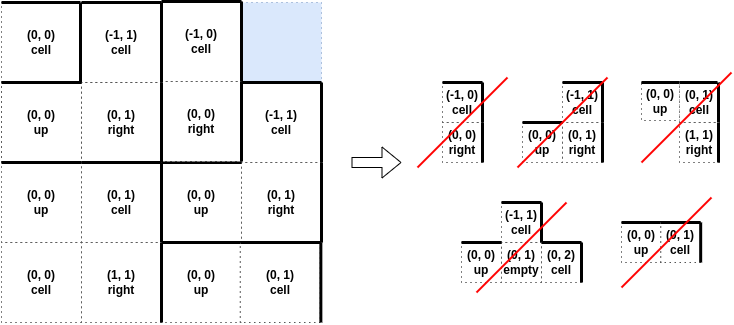
\includegraphics[scale=0.375]{img/paso7.png}
            \caption{\textbf{7.} Cambiamos a la cuarta columna y escogemos la única casilla restante. Al estar vacío el conjunto de piezas válidas, rellenamos la casilla por defecto con una celda completa.}
        \end{figure}
    \end{frame}
    
    \begin{frame}{Generación de laberintos - Modelo simple \scriptsize{\hfill \secname}}
        \begin{figure}[H]
        \centering
            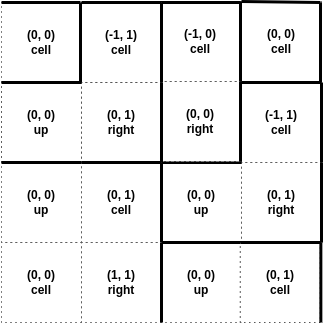
\includegraphics[scale=0.375]{img/paso8.png}
            \caption{\textbf{8.} Hemos terminado de rellenar la matriz 4x4.}
        \end{figure}
    \end{frame}
    
    \begin{frame}{Generación de laberintos - Modelo simple \scriptsize{\hfill \secname}}
        \begin{figure}[H]
        \centering
            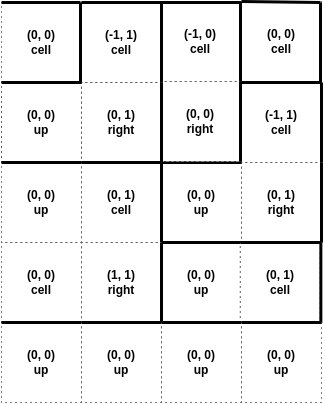
\includegraphics[scale=0.375]{img/paso9.png}
            \caption{\textbf{9.} Para finalizar el modelo simple añadiremos una fila de celdas con borde superior en la parte inferior de nuestra matriz.}
        \end{figure}
    \end{frame}
    
    \begin{frame}{Generación de laberintos - Modelo de caminos \scriptsize{\hfill \secname}}
        \begin{figure}[H]
        \centering
        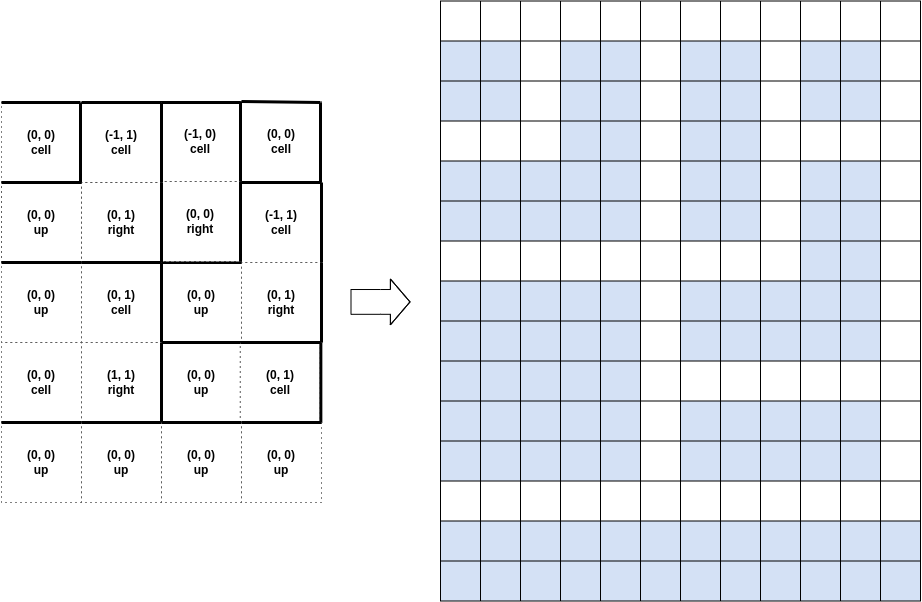
\includegraphics[scale=0.275]{img/paso10.png}
        \caption{\textbf{10.} Transformamos el modelo simple aplicando las equivalencias de celdas simples a casillas 3x3, dando como resultado una nueva matriz de tamaño 15x12.}
        \end{figure}
    \end{frame}
    
    \begin{frame}{Generación de laberintos - Modelo de caminos \scriptsize{\hfill \secname}}
        \begin{figure}[H]
        \centering
            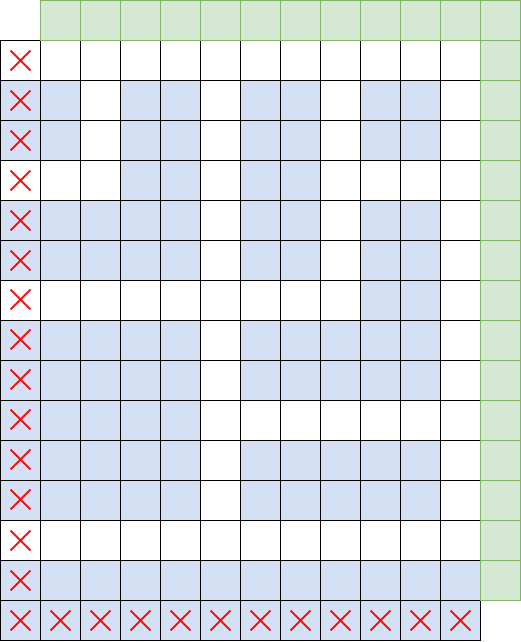
\includegraphics[scale=0.275]{img/paso11.png}
            \caption{\textbf{11.} Eliminamos la primera columna y la última fila de la matriz resultante. Además, añadimos una fila al principio y una columna al final compuestas exclusivamente de muro.}
        \end{figure}
    \end{frame}
    
    \begin{frame}{Generación de laberintos - Modelo de caminos \scriptsize{\hfill \secname}}
        \begin{figure}[H]
        \centering
            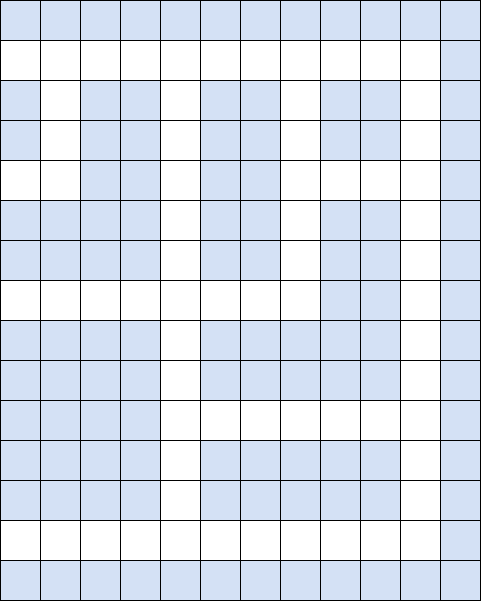
\includegraphics[scale=0.275]{img/paso12.png}
            \caption{\textbf{12.} Con estas transformaciones y modificaciones hemos completado el modelo de caminos, obteniendo una matriz de tamaño 15x12 compuesta por caminos y muros.}
        \end{figure}
    \end{frame}
    
    \begin{frame}{Generación de laberintos - Modelo final \scriptsize{\hfill \secname}}
        \begin{figure}[H]
        \centering
            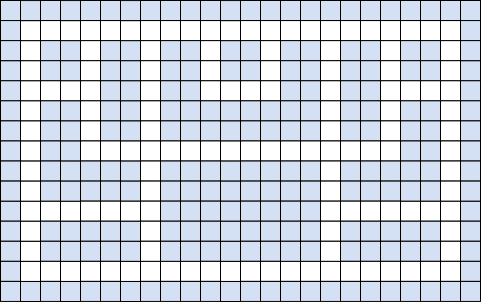
\includegraphics[scale=0.475]{img/paso13.png}
            \caption{\textbf{13.} Realizamos la simetría respecto al eje Y hacia la izquierda, obteniendo una matriz de 30x15 que forma un laberinto cerrado y válido.}
        \end{figure}
    \end{frame}
    
    \begin{frame}{Generación de laberintos - Modelo final \scriptsize{\hfill \secname}}
        \begin{figure}[H]
        \centering
            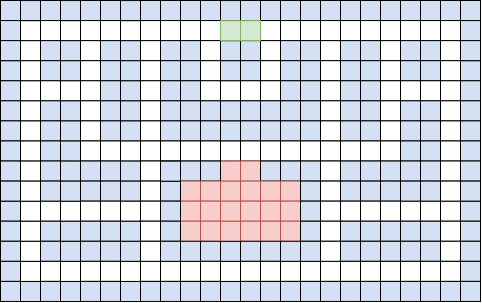
\includegraphics[scale=0.475]{img/paso14.png}
            \caption{\textbf{14.} Realizamos modificaciones para añadir o quitar muros, como por ejemplo, eliminamos los muros de la zona de la casa de los fantasmas.}
        \end{figure}
    \end{frame}
    
    \begin{frame}{Generación de laberintos - Modelo final \scriptsize{\hfill \secname}}
        \begin{figure}[H]
        \centering
            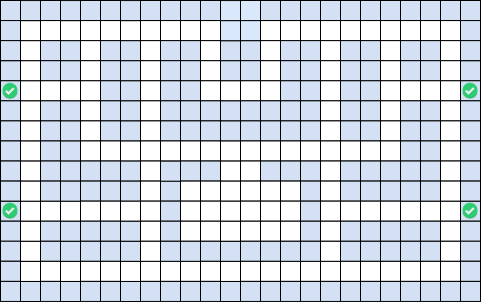
\includegraphics[scale=0.475]{img/paso15.png}
            \caption{\textbf{15.} En el caso de que no se hayan generado callejones sin salida, seleccionamos los posibles candidatos para la generación de portales, asegurando así que habrá al menos un portal.}
        \end{figure}
    \end{frame}
    
    \begin{frame}{Generación de laberintos - Modelo final \scriptsize{\hfill \secname}}
        \begin{figure}[H]
        \centering
            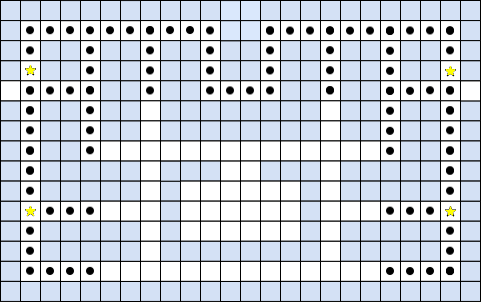
\includegraphics[scale=0.475]{img/paso16.png}
            \caption{\textbf{16.} Colocamos los puntos dejando una zona libre alrededor de la casa de los fantasmas. Añadimos los potenciadores o pastillas en las cuatro esquinas del mapa.}
        \end{figure}
    \end{frame}
    
    \begin{frame}{Generación de laberintos - Modelo final \scriptsize{\hfill \secname}}
        \begin{figure}[H]
        \centering
            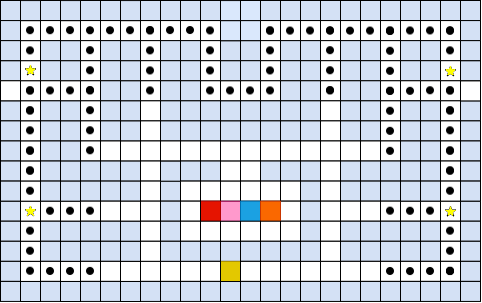
\includegraphics[scale=0.475]{img/paso17.png}
            \caption{\textbf{17.} Con ello ya dispondríamos de una matriz \textit{MazeData} compuesta por muros, caminos, puntos, pastillas y portales, y que podremos traducir a un nivel generado procedimentalmente del juego \textit{Pac-Man}.}
        \end{figure}
    \end{frame}
    
    \begin{frame}{Generación de texturas \scriptsize{\hfill \secname}}
    
        \textbf{Teselación de Voronoi}
    
        \begin{table}[H]
        \centering
            \begin{tabular}{|l|l|l|}
                \hline
                \textbf{Variable} & \textbf{Rango de valores}                                                         & \textbf{Consecuencia}                     \\ \hline
                vecA     & \begin{tabular}[c]{@{}l@{}}{[}75.0,150.0)\\ {[}200.0,350.0)\end{tabular} & Modifica el patrón               \\ \hline
                vecB     & \begin{tabular}[c]{@{}l@{}}{[}75.0,150.0)\\ {[}200.0,350.0)\end{tabular} & Modifica el patrón               \\ \hline
                amount   & {[}0.25, 0.5)                                                            & Modifica el tamaño de las celdas \\ \hline
                Hue      & {[}0.0, 1.0)                                                             & Modifica el color                \\ \hline
            \end{tabular}
        \end{table}
        
    \end{frame}
    
   \begin{frame}{Generación de texturas \scriptsize{\hfill \secname}}
    
        \begin{center}
            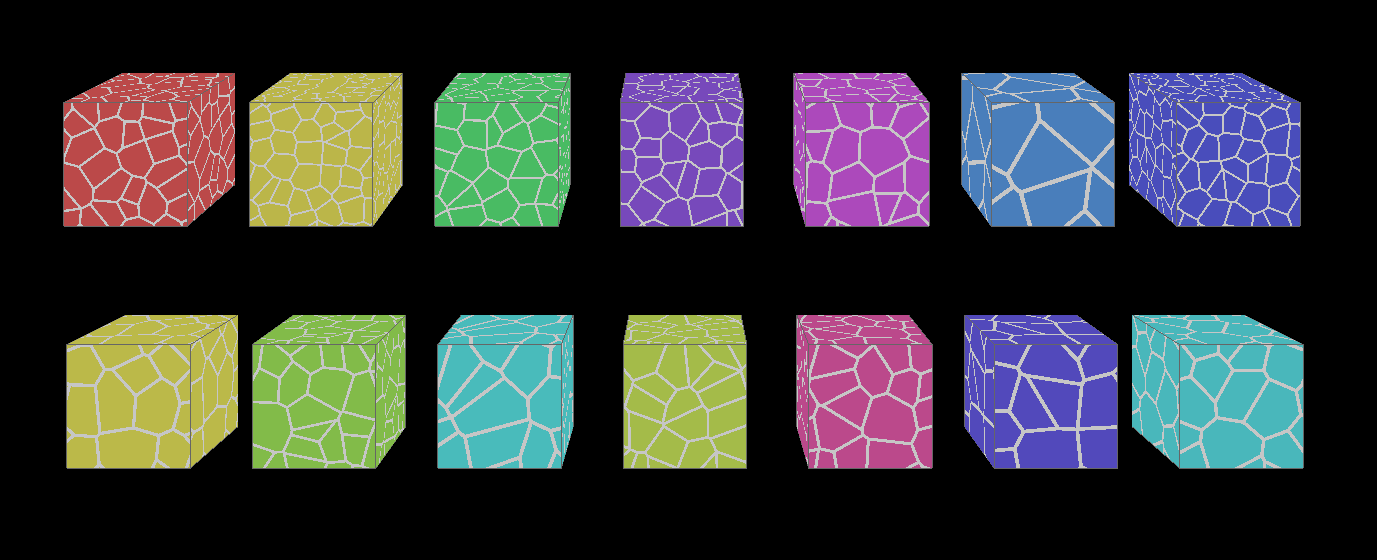
\includegraphics[scale=0.225]{img/texturas.png}
        \end{center}
        
    \end{frame}
    
   \begin{frame}{Comportamiento de la IA \scriptsize{\hfill \secname}}
    
        \begin{figure}[H]
            \begin{center}
                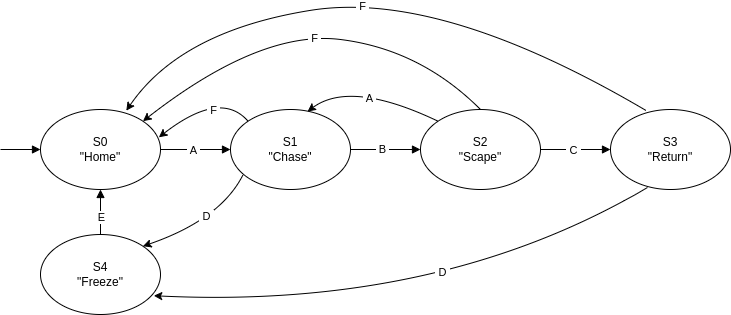
\includegraphics[scale=0.4]{img/estado_fantasmas.png}
            \end{center}
        \end{figure}   
        
    \end{frame}
    
   \begin{frame}{Comportamiento de la IA \scriptsize{\hfill \secname}}
        \footnotesize{
        \begin{table}[H]
            \centering
            \begin{tabular}{|l|l|l|l|l|}
                \hline
                \textbf{Variable}                                                         & \begin{tabular}[c]{@{}l@{}}\textbf{Valor}\\ \textbf{inicial}\end{tabular} & \begin{tabular}[c]{@{}l@{}}\textbf{Decremento}\\ \textbf{por nivel}\end{tabular} & \begin{tabular}[c]{@{}l@{}}\textbf{Valor}\\ \textbf{mínimo}\end{tabular} & \textbf{Efecto}                                                                                                                     \\ \hline
                \begin{tabular}[c]{@{}l@{}}Tiempo\\ en casa\end{tabular}         & 5s                                                      & 0.1s                                                           & 3s                                                     & \begin{tabular}[c]{@{}l@{}}Menos tiempo sin los cuatro\\ fantasmas en pantalla\end{tabular}                                \\ \hline
                \begin{tabular}[c]{@{}l@{}}Tiempo\\ asustado\end{tabular}        & \begin{tabular}[c]{@{}l@{}}10s\\ +5s\end{tabular}       & 0.5s                                                           & \begin{tabular}[c]{@{}l@{}}0.1s\\ +5s\end{tabular}     & \begin{tabular}[c]{@{}l@{}}Menor ventana de tiempo para\\ eliminar a los enemigos\end{tabular}                             \\ \hline
                \begin{tabular}[c]{@{}l@{}}Tiempo\\ entre\\ caminos\end{tabular} & 7.5s                                                    & 0.2s                                                           & 2s                                                     & \begin{tabular}[c]{@{}l@{}}Mayor agresividad y precisión\\ de los enemigos a la hora de\\ localizar a Pac-Man\end{tabular} \\ \hline
            \end{tabular}
        \end{table}
        }
        
    \end{frame}

\section{Conclusiones}

    \begin{frame}{Resultados \scriptsize{\hfill \secname}}
    
        \begin{itemize}
            \item Buena primera aproximación a la generación procedimental de contenidos, especialmente en el ámbito de los videojuegos.
            \item Juego original fielmente reproducido, añadiendo un enfoque personal.
            \item Resolución de conflictos a bajo nivel durante el desarrollo.
            \item Gestión y ejecución adecuada de un proyecto software completo.
        \end{itemize}
    
    \end{frame}

    \begin{frame}{Resultados \scriptsize{\hfill \secname}}
    
        \begin{itemize}
            \item Empleadas técnicas de generación procedimental de contenido a los laberintos (\textit{Game Space}) y texturas del juego (\textit{Game Bits}).
            \item Añadida dificultad adaptativa, complementando a estas técnicas.
            \item Los algoritmos diseñados cumplen con cuatro de las cinco propiedades deseables: velocidad, fiabilidad, diversidad y credibilidad.
        \end{itemize}
    
    \end{frame}
    
    \begin{frame}{Ejemplos \scriptsize{\hfill \secname}}
        \centering
        \vspace{3mm}
        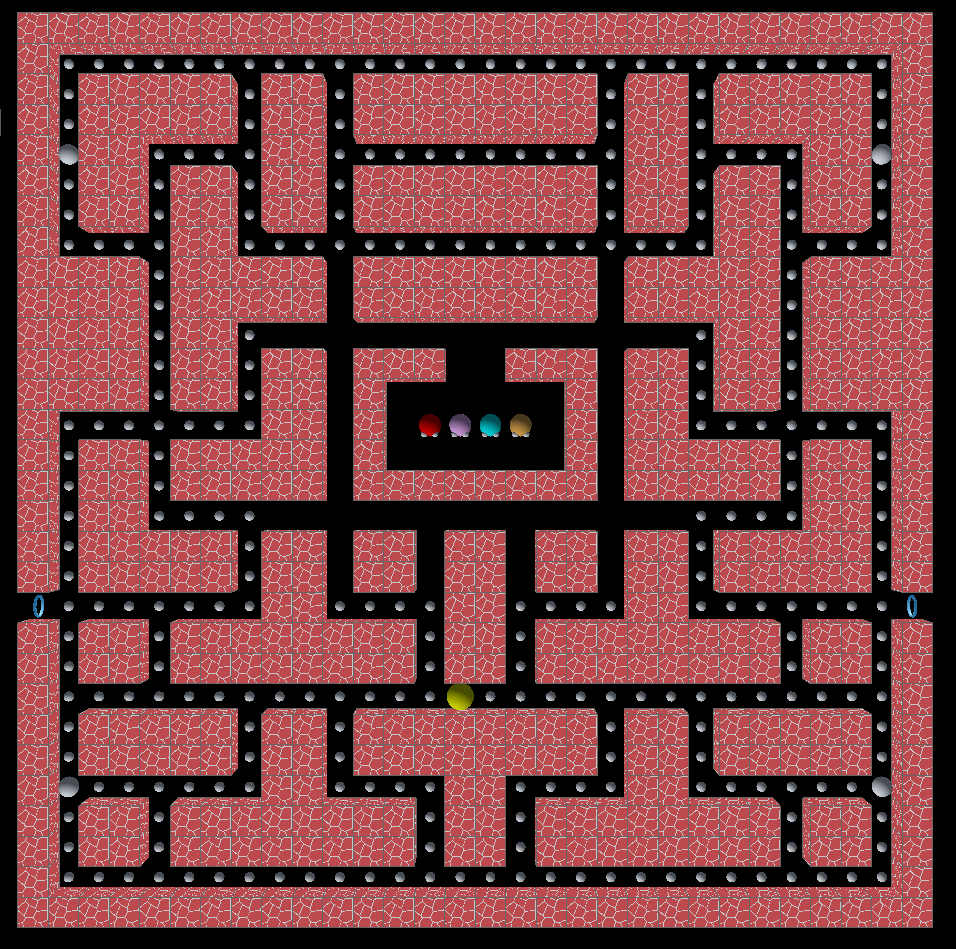
\includegraphics[scale=0.15]{img/laberinto1.png}
        \hspace{3mm}
        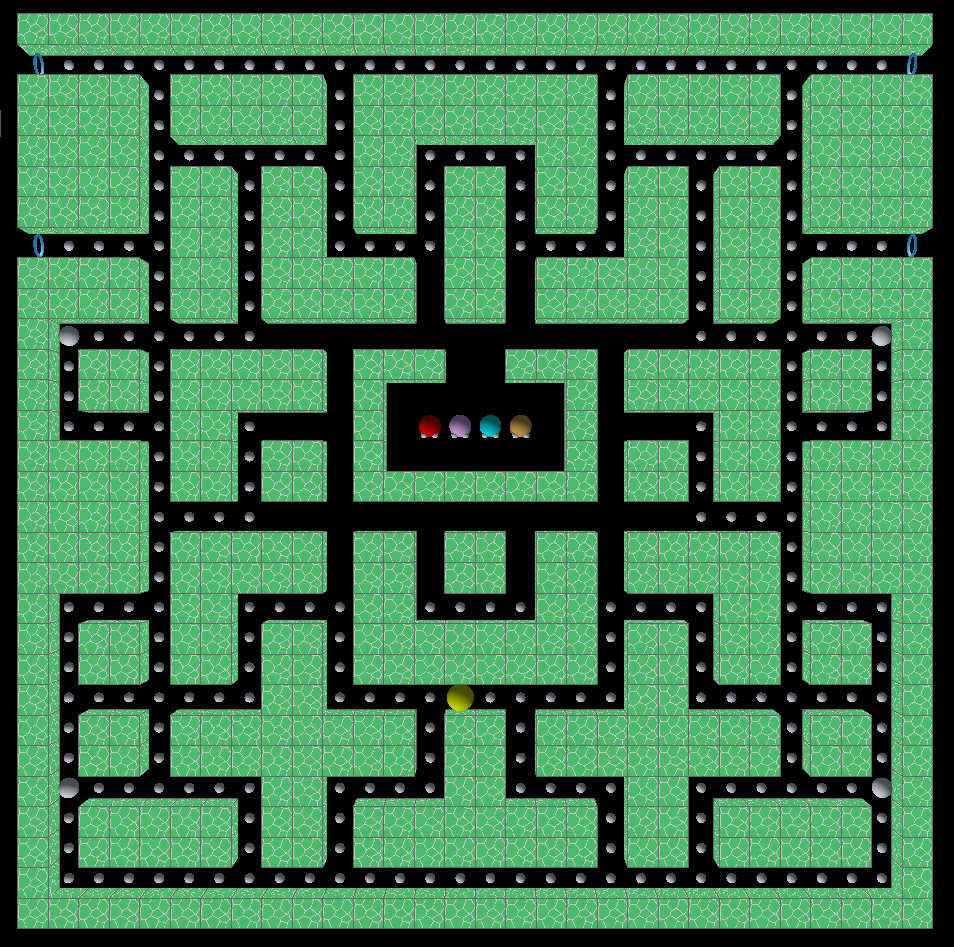
\includegraphics[scale=0.15]{img/laberinto2.png}
    \end{frame}
    
    \begin{frame}{Ejemplos \scriptsize{\hfill \secname}}
        \centering
        \vspace{3mm}
        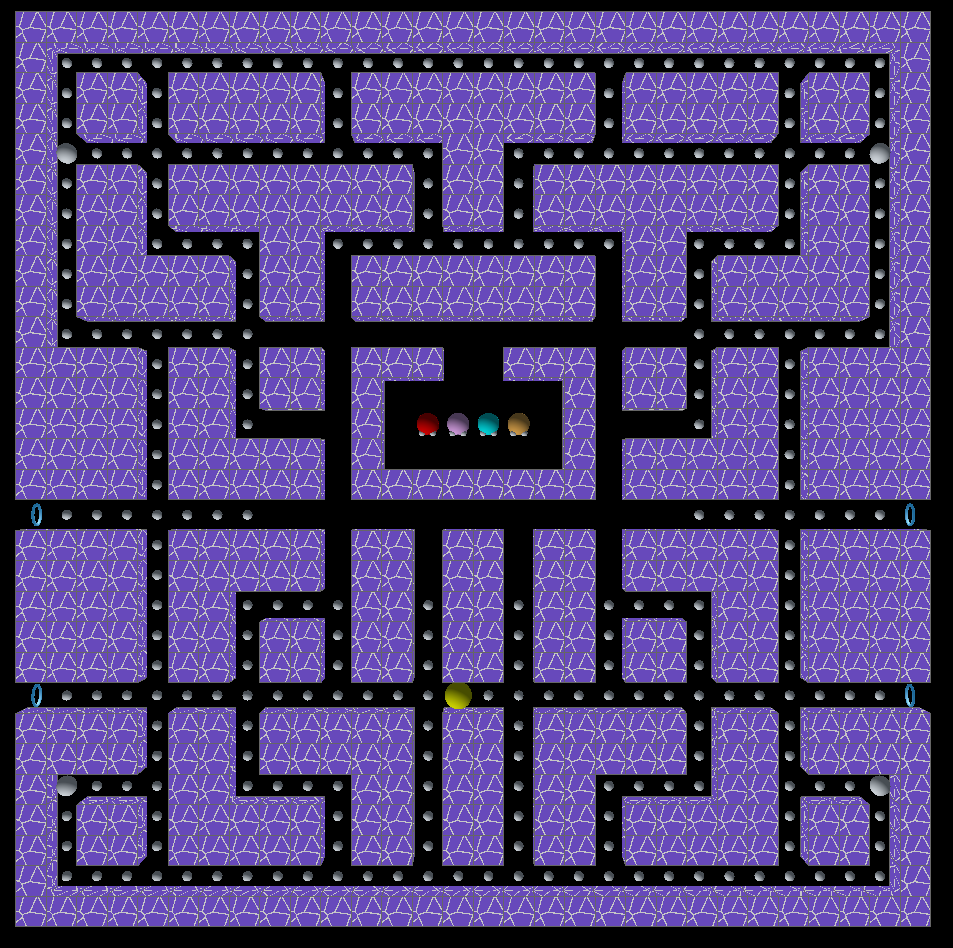
\includegraphics[scale=0.15]{img/laberinto3.png}
        \hspace{3mm}
        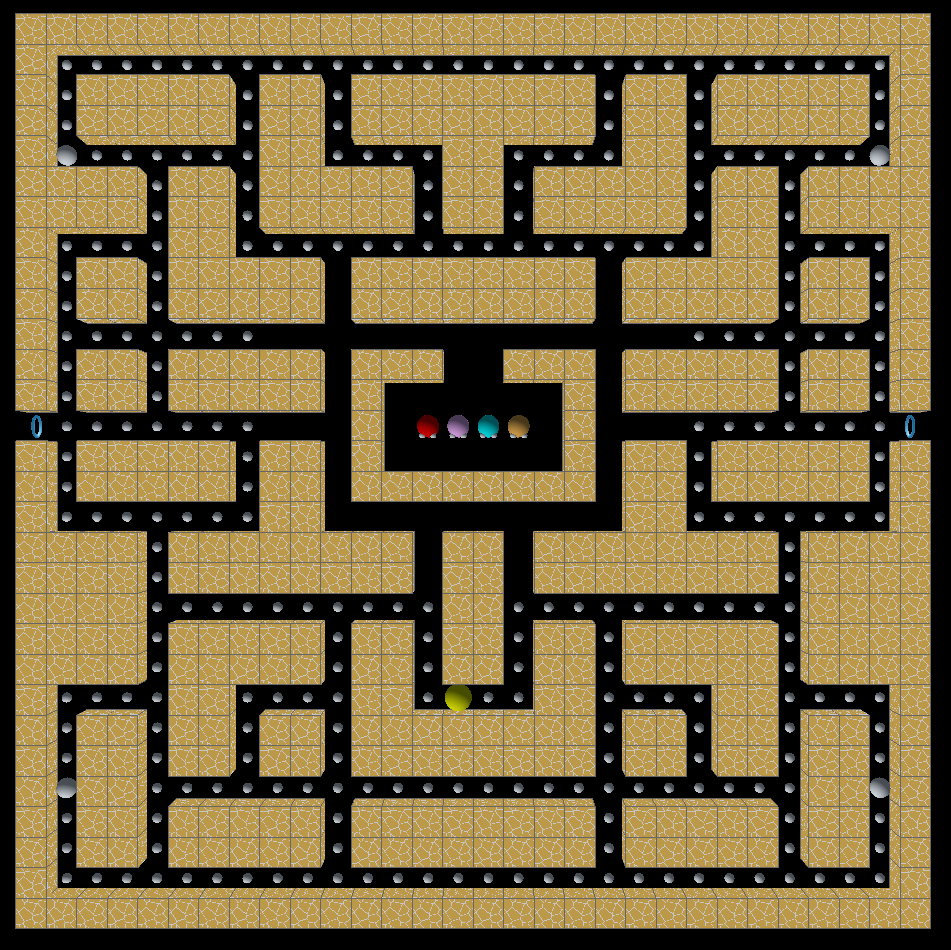
\includegraphics[scale=0.15]{img/laberinto4.png}
    \end{frame}
    
    \begin{frame}{Ejemplos \scriptsize{\hfill \secname}}
        \centering
        \vspace{3mm}
        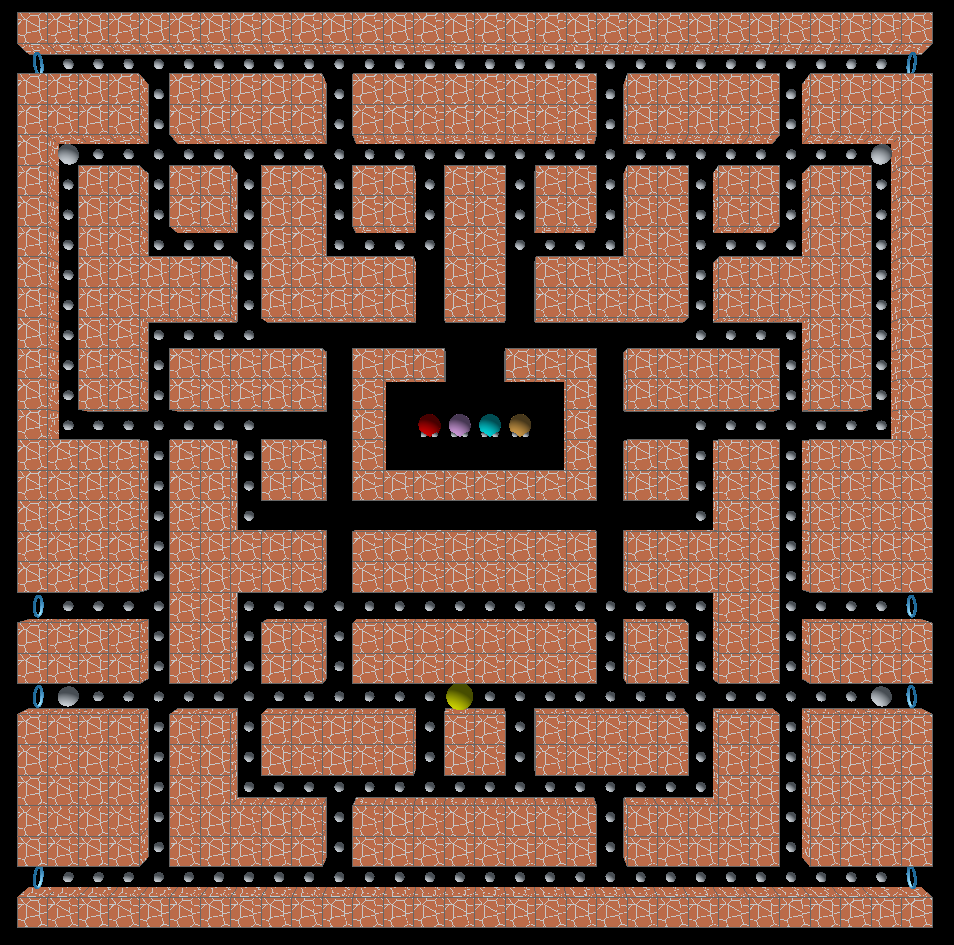
\includegraphics[scale=0.15]{img/laberinto5.png}
        \hspace{3mm}
        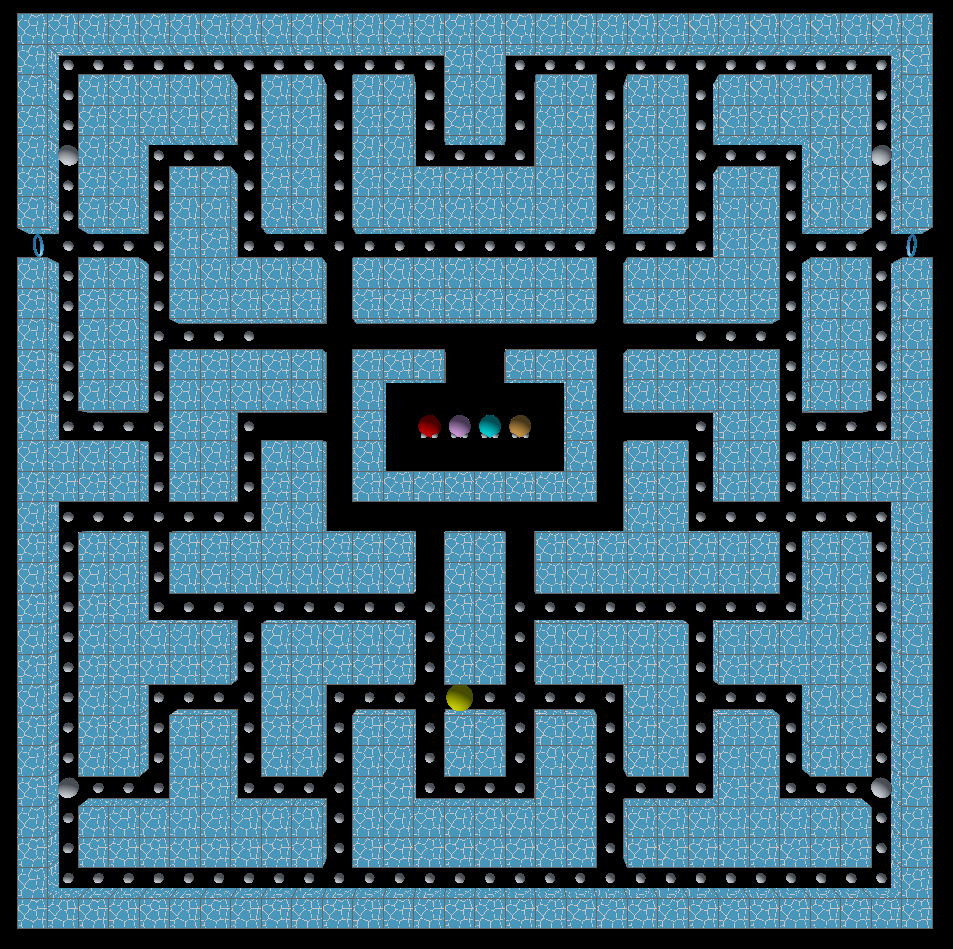
\includegraphics[scale=0.15]{img/laberinto6.png}
    \end{frame}

    \begin{frame}{Trabajos futuros \scriptsize{\hfill \secname}}
    
        \begin{itemize}
            \item Realizar mejoras a nivel de aplicación.
            \item Continuar ampliando conocimientos sobre generación procedimental de contenidos.
            \begin{itemize}
                \item Implementar semillas en el algoritmo de generación de laberintos.
                \item Combinar el algoritmo implementado con métodos basados en búsqueda.
                \item Estudiar otras técnicas, en particular, el algoritmo de colapso de la función de onda.
            \end{itemize}
        \end{itemize}
        
    \end{frame}

\section{Referencias}

    \begin{frame}{Tecnologías utilizadas \scriptsize{\hfill \secname}}
    
    	\begin{table}[H]
    	\centering
    	\resizebox{\textwidth}{!}{%
    	\begin{tabular}{cc}
    	
\includegraphics[width=0.225\textwidth]{img/git.png} & 
\includegraphics[width=0.275\textwidth]{img/github.png} \\
    	
\includegraphics[width=0.3\textwidth]{img/githubPages.png} & 
    	
\includegraphics[width=0.22\textwidth]{img/threejs.png} 
    	\end{tabular}%
    	}
    	\end{table}
    
    \end{frame}

    \begin{frame}{Bibliografía \scriptsize{\hfill \secname}}
        \begin{thebibliography}{1}
        
        %--------- #A ---------%
    
        \bibitem[Amato, 2017]{amato2017}
    	
    	[Amato, 2017] \href{https://doi.org/10.1007/978-3-319-53088-8_2}{Amato, A. (2017). Procedural content generation in the game industry. En O. Korn \& N. Lee (Eds.), Game Dynamics (pp. 15-25). Springer International Publishing.}
        
        %--------- #B ---------%
        
        \bibitem[Barriga, 2019]{barriga2019}
    	
    	[Barriga, 2019] \href{https://doi.org/10.1142/S0218213019300011}{Barriga, N. A. (2019). A short introduction to procedural content generation algorithms for videogames. International Journal on Artificial Intelligence Tools, 28(02), 1930001.}
    	
    	\bibitem[Breda University, 2021]{EP}
    	
    	[Breda University, 2021] \href{http://everythingprocedural.com/}{Breda University of Applied Sciences. (2021). EPC2021—Everything Procedural Conference.}
        
        \end{thebibliography}
    \end{frame}
    
    \begin{frame}{Bibliografía \scriptsize{\hfill \secname}}
        \begin{thebibliography}{1}
        
        %--------- #C ---------%
    	\bibitem[Cabello, s.f.]{three.js}
    	
    	[Cabello, s.f.] \href{https://threejs.org/}{Cabello, R. ``Mr.doob'' (2021). Three.js – JavaScript 3D Library.}
    	
    	%--------- #H ---------%
    	
    	\bibitem[Hendrikx et al., 2013]{hendrikx2013}
    	
    	[Hendrikx et al., 2013] \href{https://doi.org/10.1145/2422956.2422957}{Hendrikx, M., Meijer, S., Van Der Velden, J., \& Iosup, A. (2013). Procedural content generation for games: A survey. ACM Transactions on Multimedia Computing, Communications, and Applications, 9(1), 1-22.}
    	
    	%--------- #L---------%
    	
    	\bibitem[LeBron, 2012]{lebron2012}
    	
        [LeBron, 2012] \href{https://shaunlebron.github.io/pacman-mazegen/}{LeBron, S. (2012). Pac-Man Maze Generation.}
        
        \end{thebibliography}
    \end{frame}
    
    \begin{frame}{Bibliografía \scriptsize{\hfill \secname}}
        \begin{thebibliography}{1}
        
        %--------- #P ---------%
    	
    	\bibitem[Pittman, 2015]{pittman2015}
    	
    	[Pittman, 2015] \href{https://pacman.holenet.info/}{Pittman, J. (2015). The Pac-Man Dossier.}
        
    	%--------- #Q ---------%
    	
    	\bibitem[Quílez, 2013]{quilez}
    	
    	[Quílez, 2013] \href{https://www.iquilezles.org/www/articles/voronoilines/voronoilines.htm}{Quílez, I. (2013). Shader example—Voronoi with borders.}
    	
    	%--------- #S ---------%
    	
    	\bibitem[Shaker et al., 2016]{shaker2016}
    	
    	[Shaker et al., 2016] \href{https://doi.org/10.1007/978-3-319-42716-4}{Shaker, N., Togelius, J., \& Nelson, M. J. (2016). Procedural content generation in games. Springer International Publishing.}
        
        \end{thebibliography}
    \end{frame}
    
    \begin{frame}{Bibliografía \scriptsize{\hfill \secname}}
        \begin{thebibliography}{1}
    	
    	\bibitem[Smith, 2015]{smith2015}
    	
    	[Smith, 2015] \href{http://sokath.com/home/wp-content/uploads/2018/01/smith-fdg15.pdf}{Smith, G. (2015). An Analog History of Procedural Content Generation. In Foundations of Digital Games.}
    	
    	%--------- #T ---------%
    	
    	\bibitem[Togelius et al., 2011]{togelius2011}
    	
    	[Togelius et al., 2011] \href{https://doi.org/10.1109/TCIAIG.2011.2148116}{Togelius, J., Yannakakis, G. N., Stanley, K. O., \& Browne, C. (2011). Search-based procedural content generation: A taxonomy and survey. IEEE Transactions on Computational Intelligence and AI in Games, 3(3), 172-186.}
        
        \end{thebibliography}
    \end{frame}

\section{Demo}

    \begin{frame}{Demo}
    \centering
    
        \begin{figure}[H]
            \begin{center}
                
\includegraphics[scale=0.15]{img/githubPages.png}
            \end{center}
        \end{figure}   
    
        \href{https://gsandoval96.github.io/TFG-UGR/pacman/src/}{https://gsandoval96.github.io/TFG-UGR/pacman/src/}
        
    \end{frame}

\end{document}